\chapter{Weekly Reports \\
\small{\textit{- Ryan Davis, Cory Vitanza, and Roy Tas}}%
}
\index{weekly reports}
\index{Chapter!Weekly Reports}
\label{Chapter::WeeklyReports}

%=======================================================
\section{Week Report 13 (12/11/2025)}
\label{sec:report13}

\subsection{Progress Made}
\begin{itemize}

    \item Connected board to SenseCraft UI for GPS testing.

    \begin{figure}[H]
        \centering
        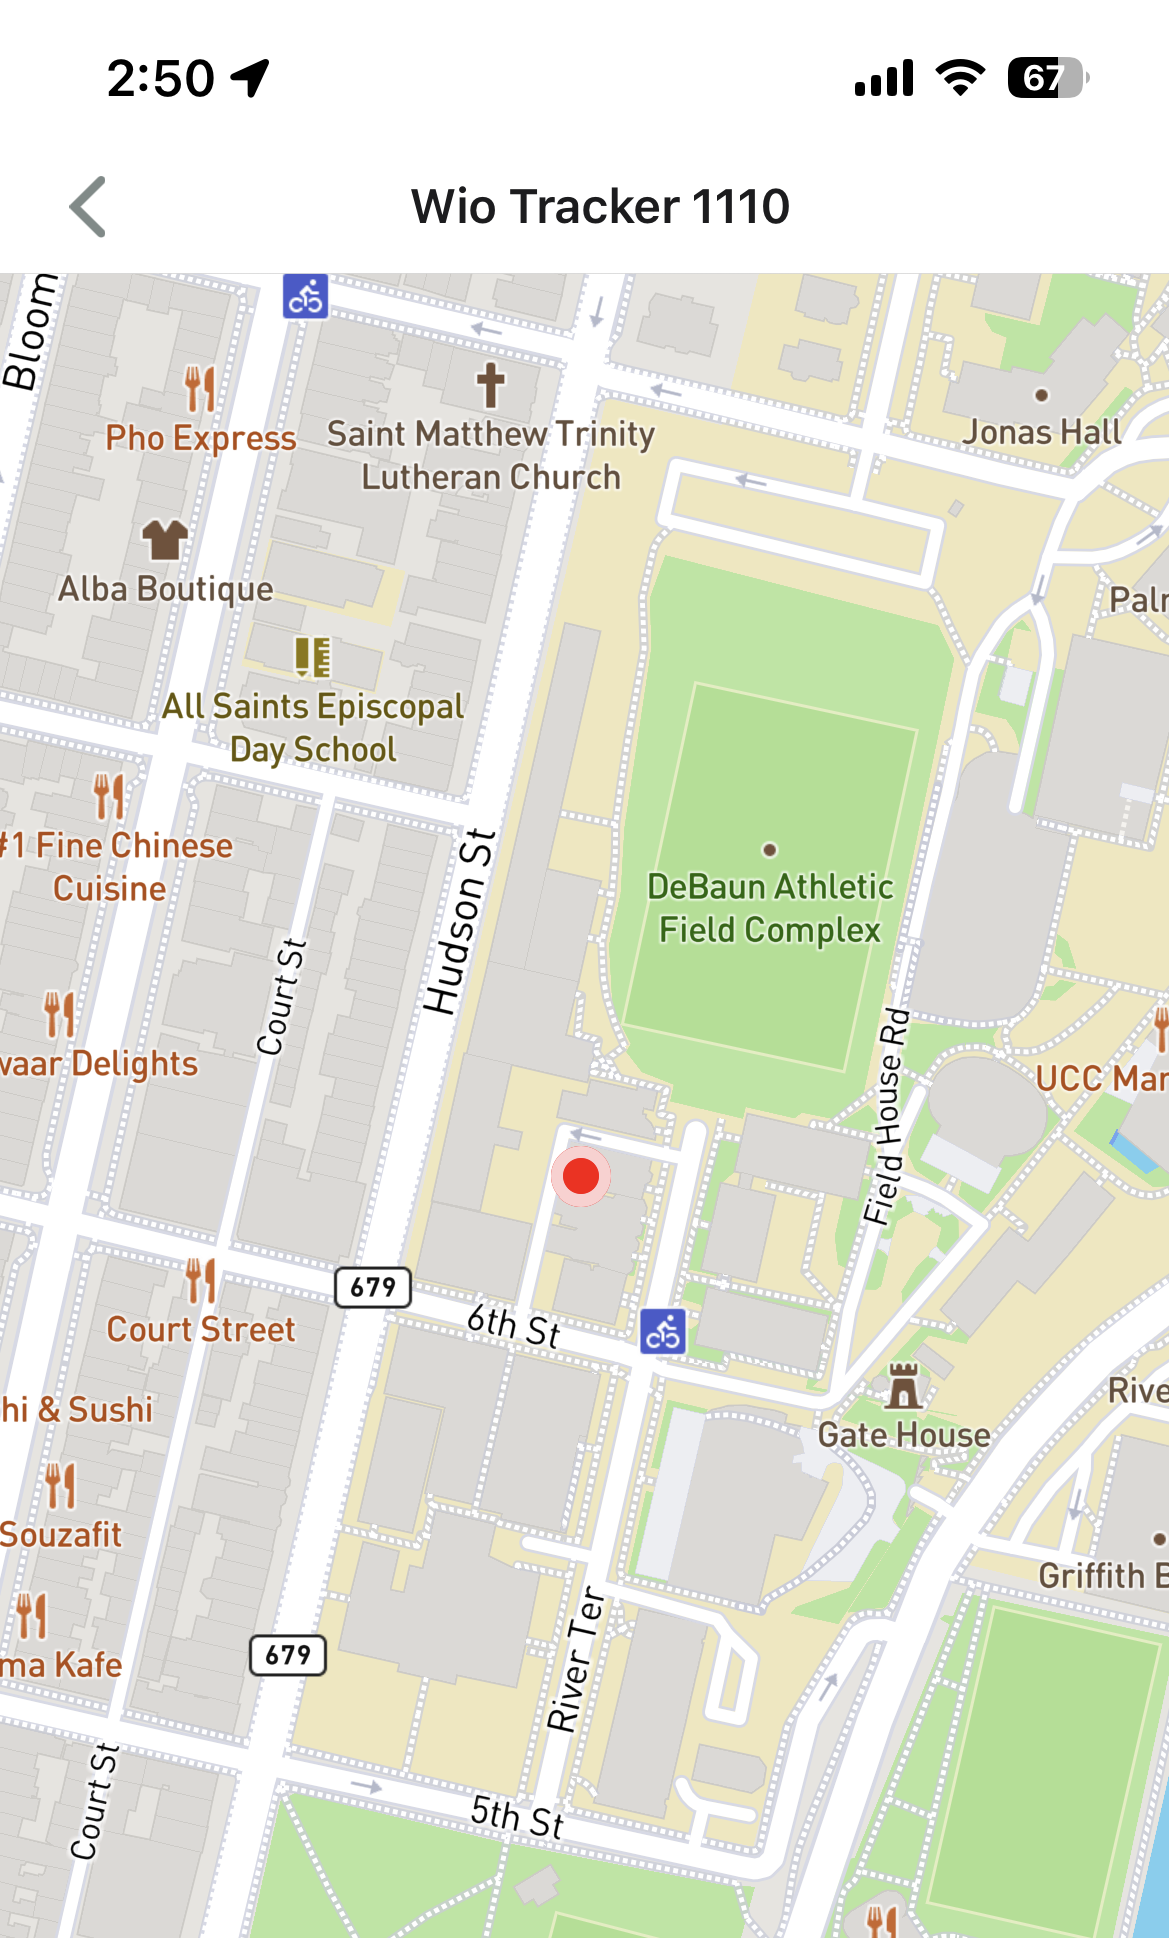
\includegraphics[width=0.7\textwidth]{png/screenshots/sensecraft.png}
        \caption{\FigureLabel{SensecraftConnection}: SenseCraft UI connection for GPS testing}
        \label{fig:SensecraftConnection}
    \end{figure}
    The screenshot above shows the device’s GPS output appearing correctly in SenseCraft.

    \item Developed authorization protocol with React Frontend and Supabase Database for user accounts.
    % Uncomment when screenshot ready:
    \begin{figure}[H]
        \centering
        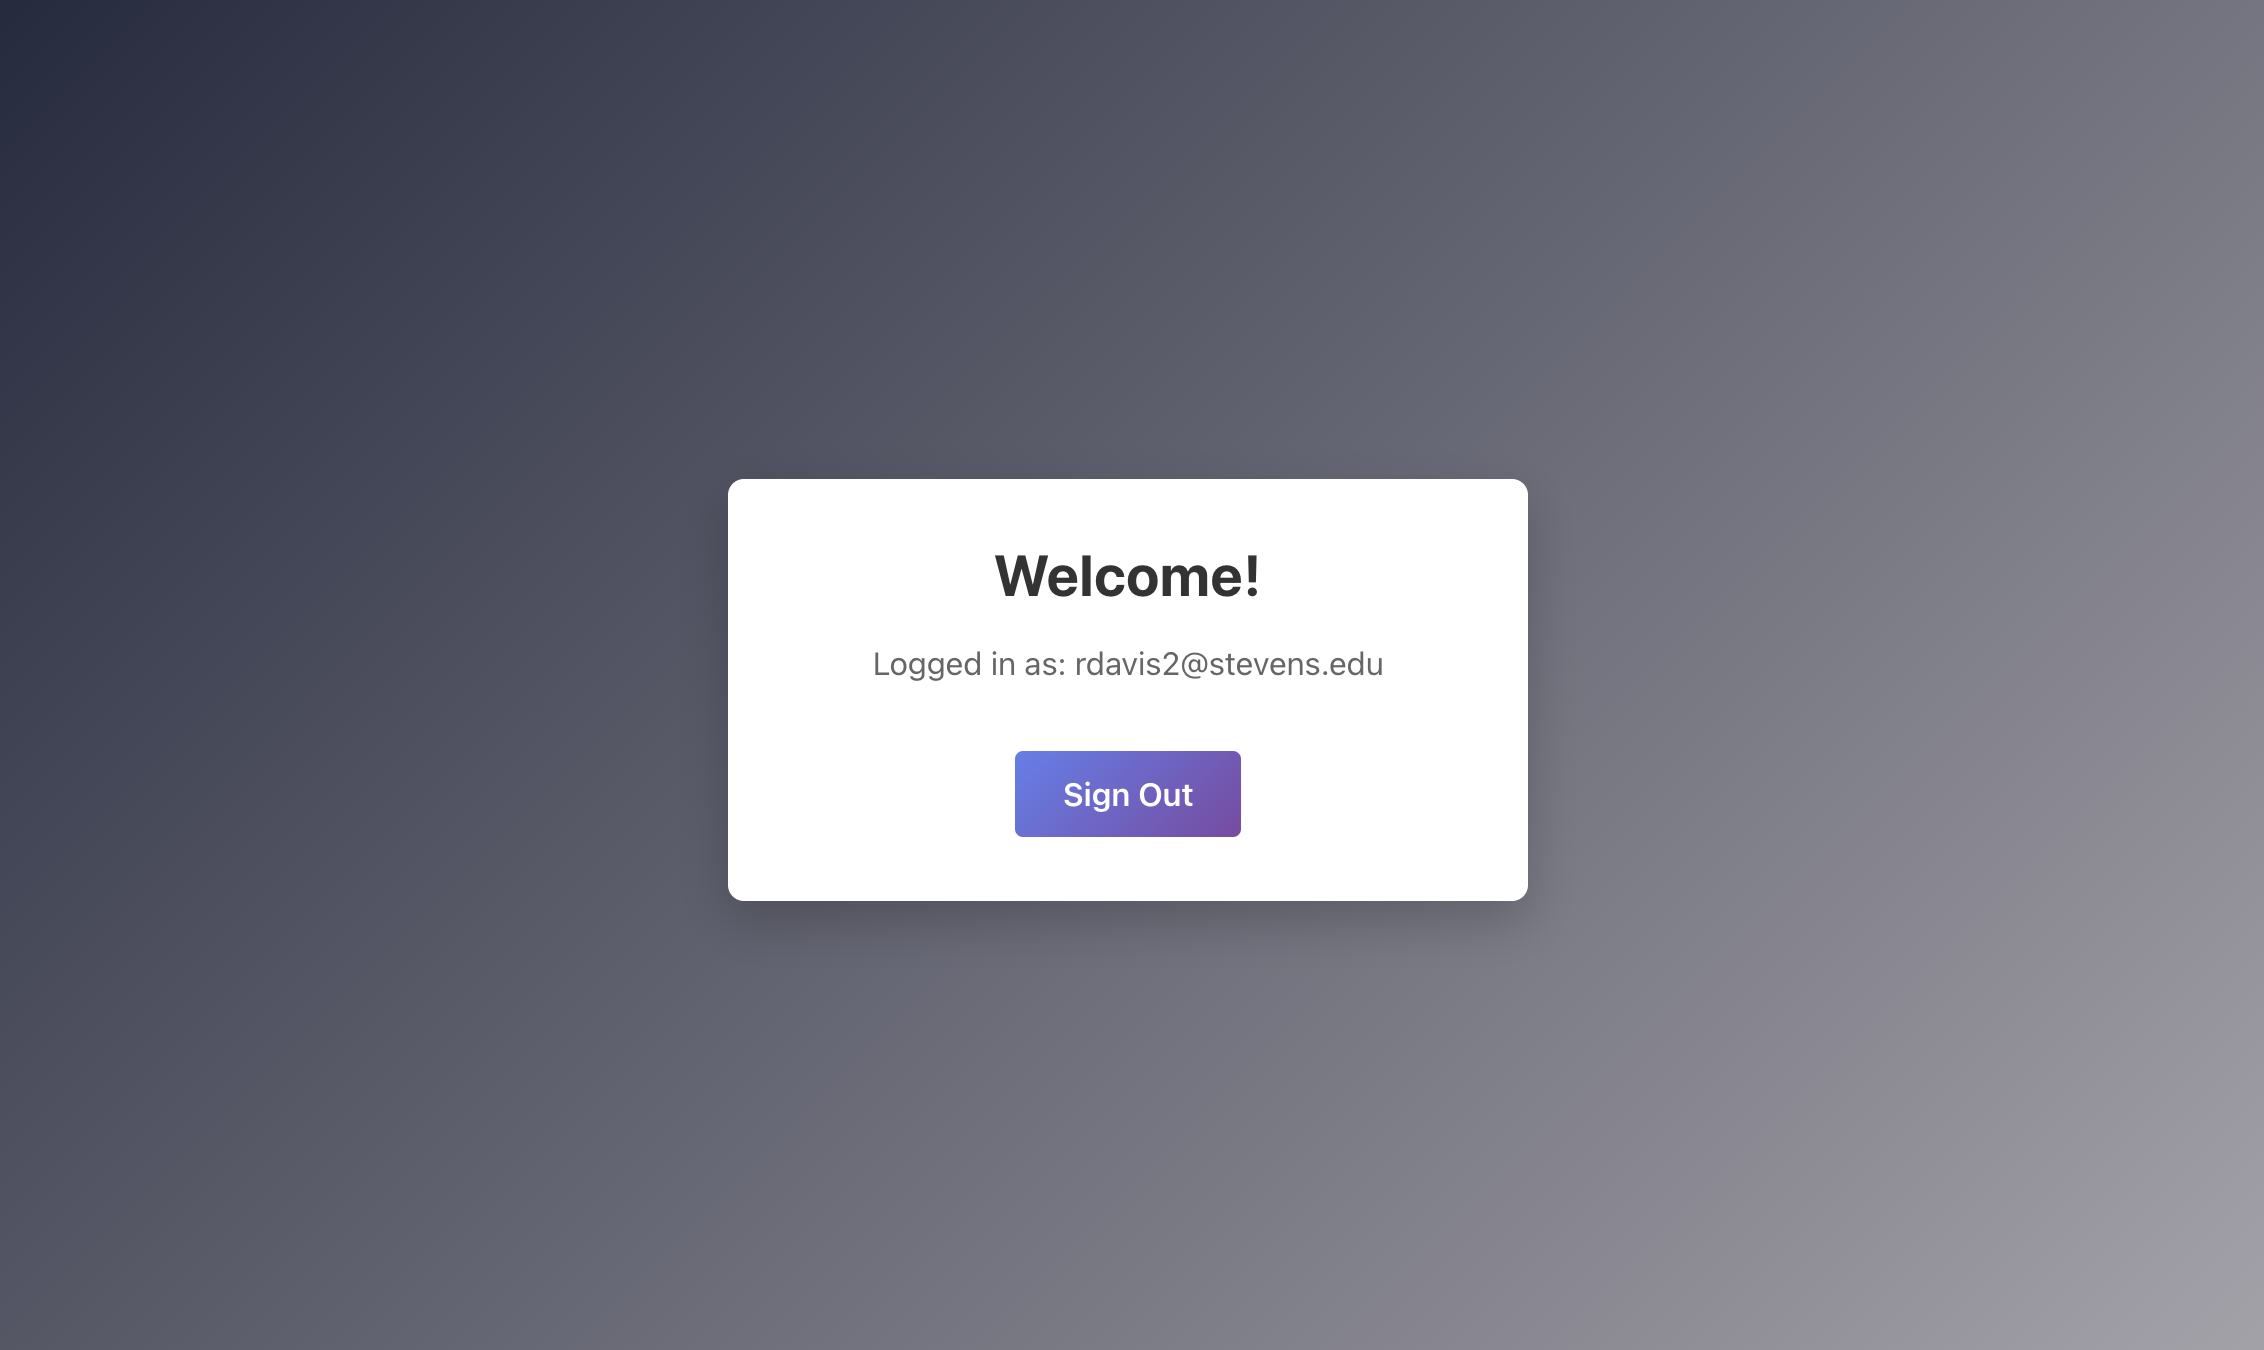
\includegraphics[width=0.7\textwidth]{png/screenshots/AuthUI.png}
        \caption{\FigureLabel{DevServer}: React development server showing authorization flow}
        \label{fig:DevServer}
    \end{figure}
    The figure above would show the login system functioning in the dev server.

    \item Established database schema for board integrations.

    \begin{figure}[H]
        \centering
        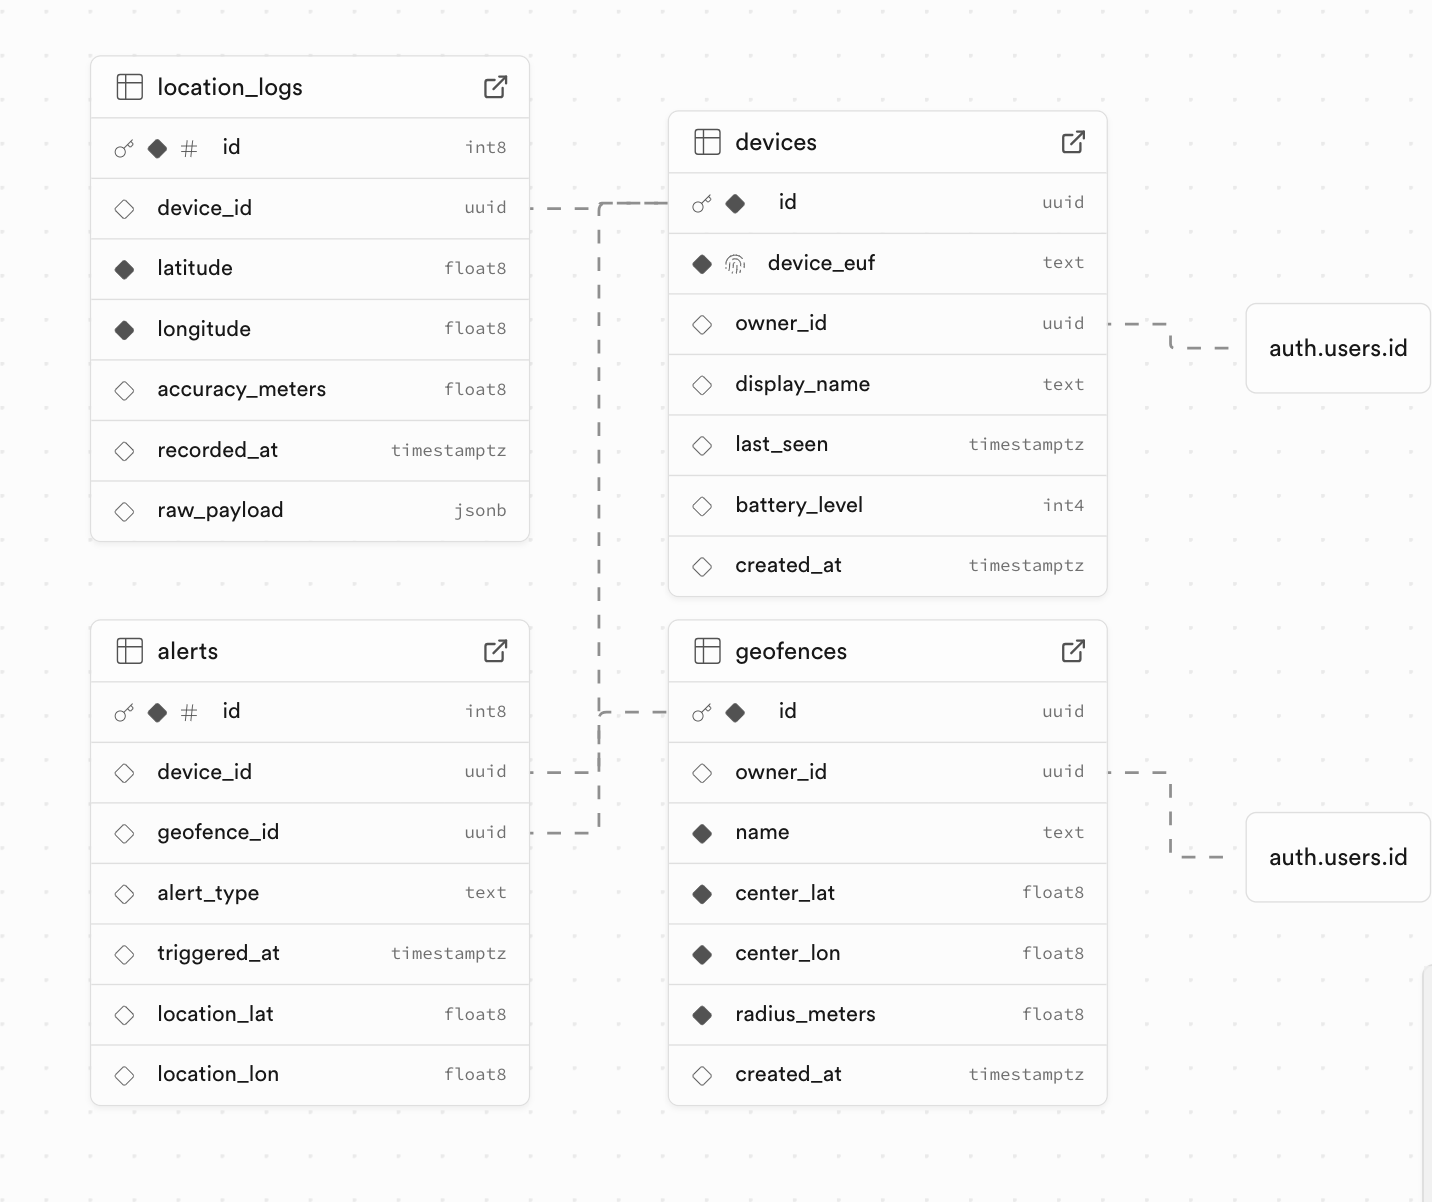
\includegraphics[width=0.7\textwidth]{png/screenshots/dbSchema.png}
        \caption{\FigureLabel{SupabaseSchema}: Supabase schema for board integration}
        \label{fig:SupabaseSchema}
    \end{figure}
    The schema diagram above shows how each device is linked to a user via \texttt{auth.users.id}.

    \item Developed a case for the Wio Tracker 1110.

    \begin{figure}[H]
        \centering
        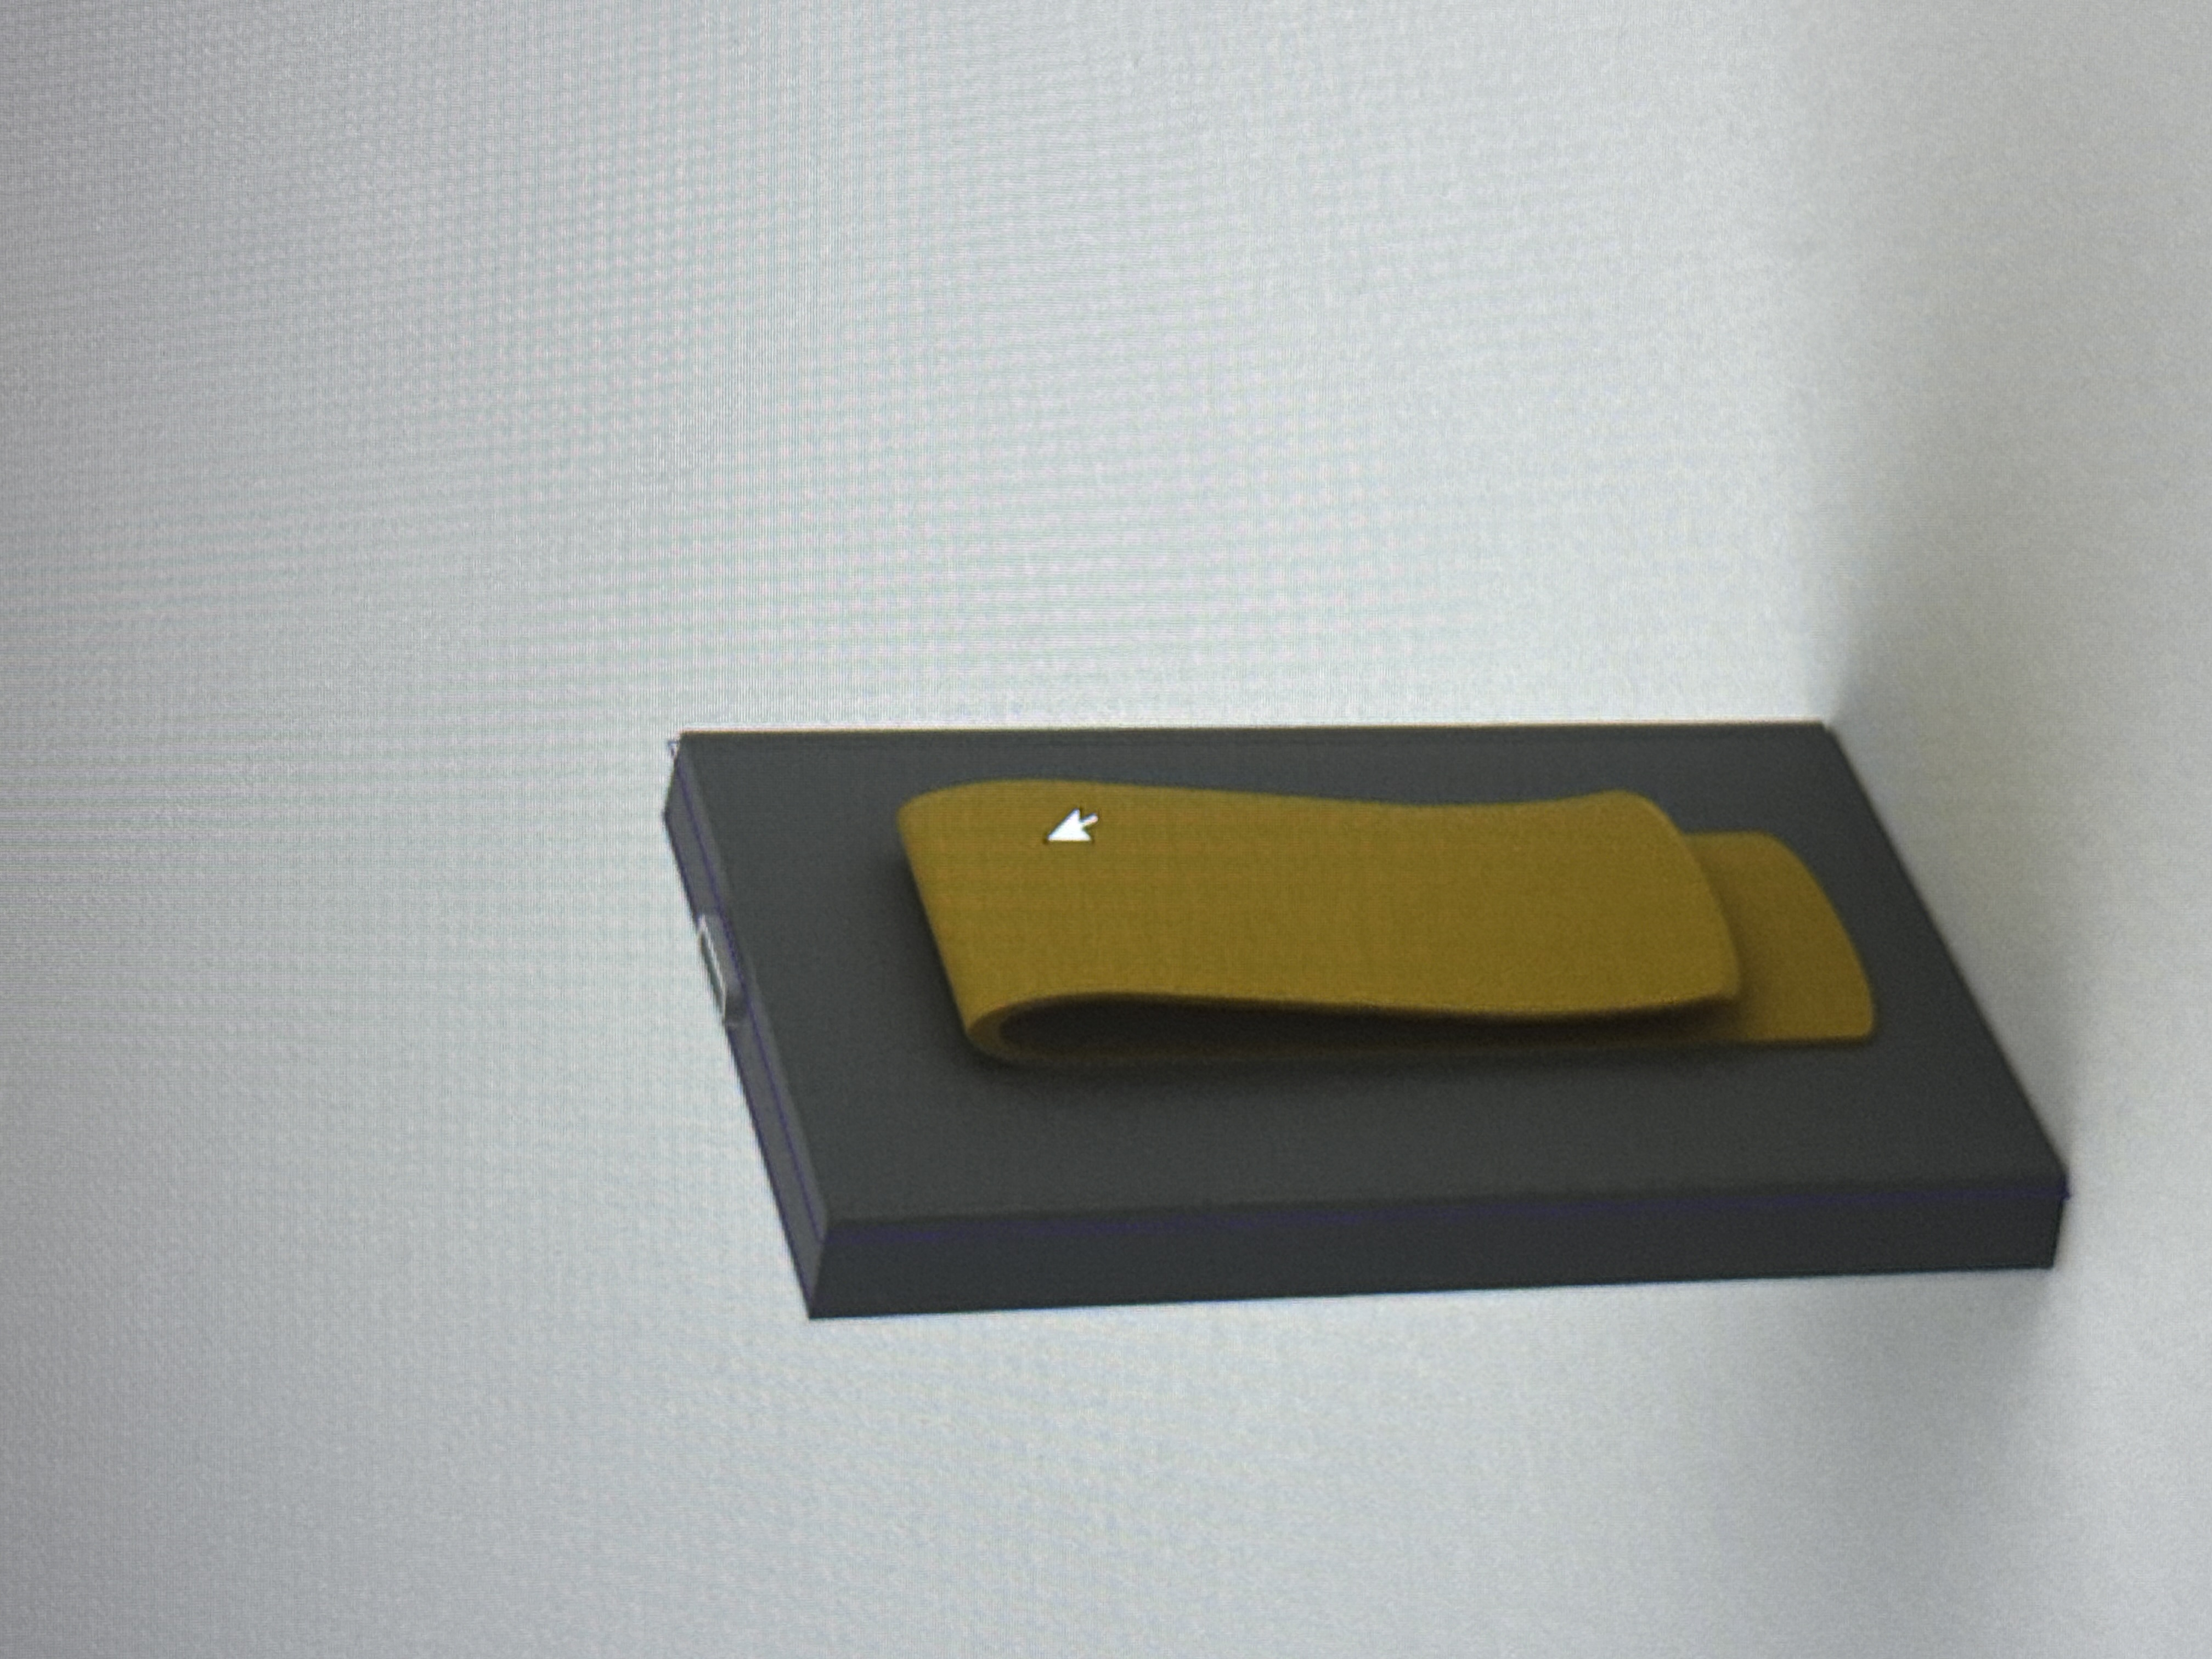
\includegraphics[width=0.7\textwidth]{png/screenshots/caseClip.png}
        \caption{\FigureLabel{CaseClip}: Clip for the Wio Tracker 1110}
        \label{fig:CaseClip}
    \end{figure}
    The clip design above demonstrates the mounting mechanism for the tracker.

    \begin{figure}[H]
        \centering
        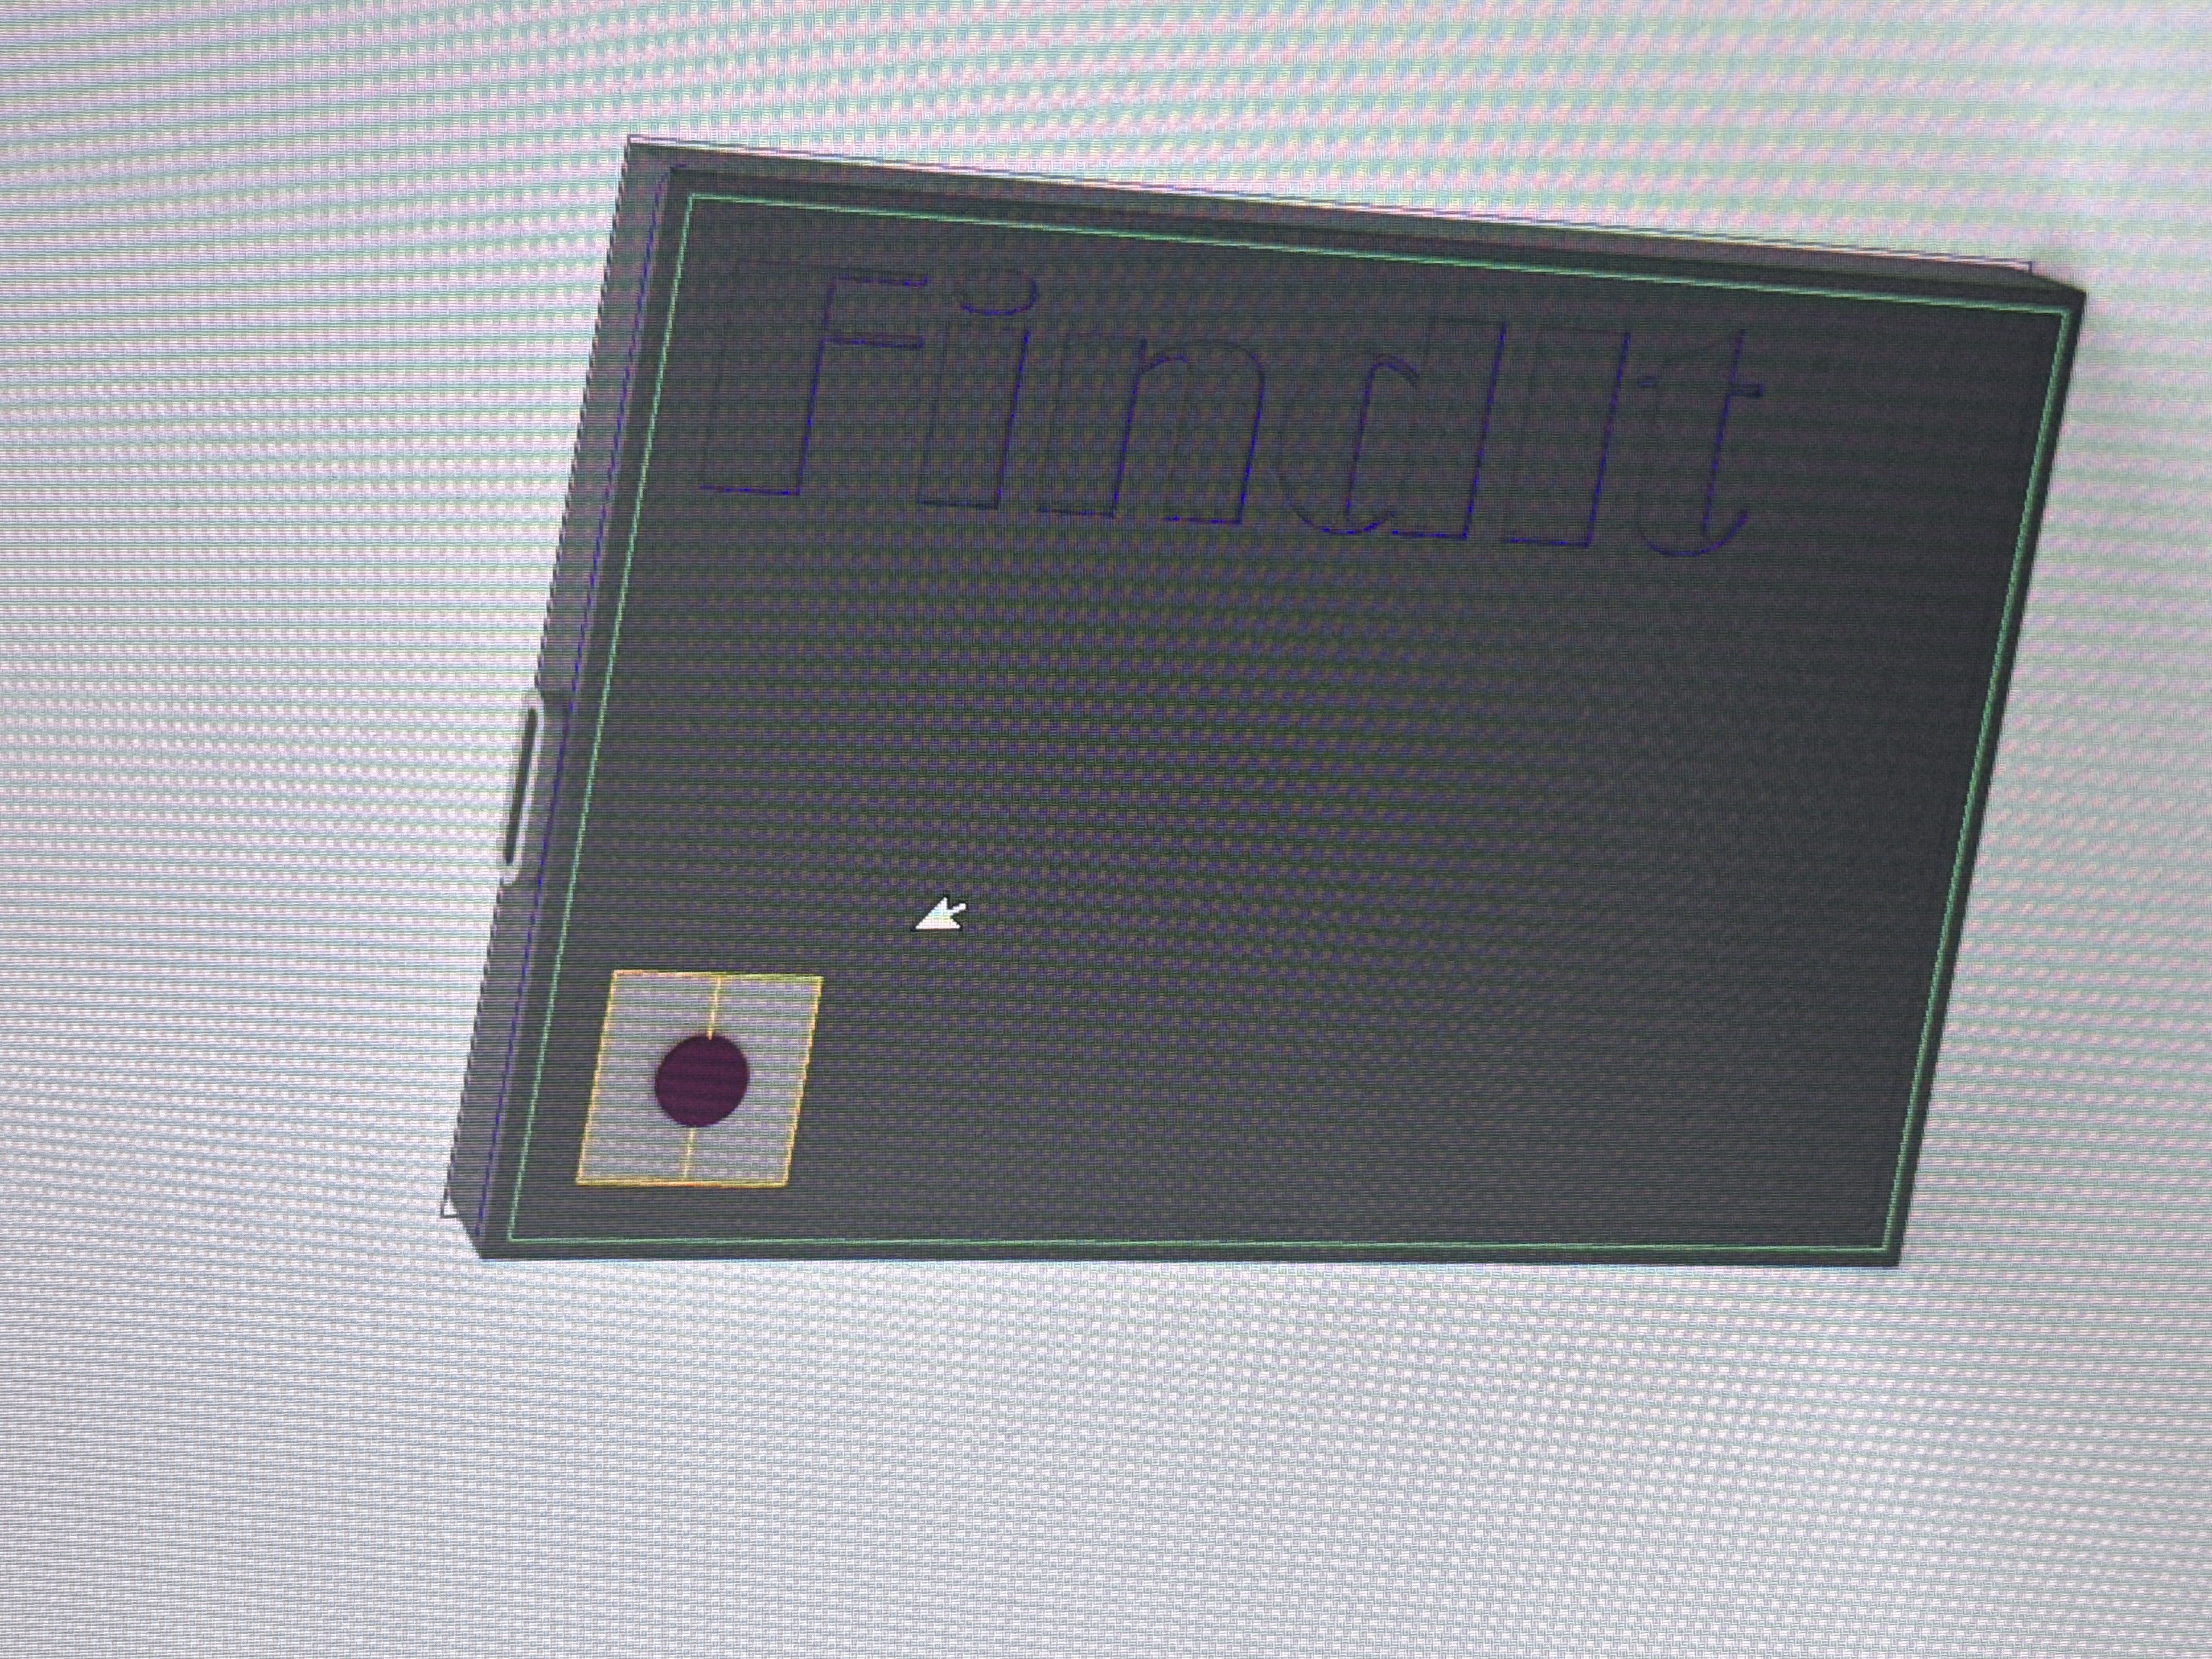
\includegraphics[width=0.7\textwidth]{png/screenshots/caseIsometric.png}
        \caption{\FigureLabel{CaseIsometric}: Isometric view of the initial case prototype}
        \label{fig:CaseIsometric}
    \end{figure}
    The isometric view above provides a full perspective of the initial enclosure prototype.

    \item Flashed board with default firmware to connect to SenseCraft UI and retrieve LoRaWAN device keys.
    % Uncomment when screenshot ready:
    %\begin{figure}[H]
    %    \centering
    %    \includegraphics[width=0.7\textwidth]{png/screenshots/serial_output.png}
    %    \caption{\FigureLabel{SerialOutput}: Serial monitor output during firmware flashing}
    %    \label{fig:SerialOutput}
    %\end{figure}
    %Serial output screenshot would appear here.

\end{itemize}

\subsection{Next Week's Plan}
\begin{itemize}
    \item Continue configuring the board to connect to the LoRaWAN network server.
    \item Implement OpenStreetMaps API in the React frontend for mapping functionality.
\end{itemize}


%=======================================================
\section{Week Report 12 (12/05/2025)}
\label{sec:report12}

\subsection{Progress Made}
\begin{itemize}
    \item Received the Wio Tracker 1110 Development Board.
    \item Configured The Things Stack LoRaWAN network.
    \item Initialized database tables and schema.
\end{itemize}

\subsection{Next Week's Plan}
\begin{itemize}
    \item Configure the development board with SenseCap to collect device keys.
    \item Debug the firmware to optimize GPS collection and confirm LoRaWAN uplinks.
    \item Prepare the React user interface for prototype demonstration.
\end{itemize}


%=======================================================
\section{Week Report 11 (11/14/2025)}
\label{sec:report11}

\subsection{Progress Made}
\begin{itemize}
    \item Created a \hyperref[fig:figmaUI]{Paper Prototype} for the FindIt user interface.
    \item Developed user personas for the \hyperref[Chapter::UserInterfaceDesign]{User Interface Design}.
    \item Began composing UML diagrams for the \hyperref[Chapter::LogicalView]{logical view} (class diagram), \hyperref[Chapter::DevelopmentView]{development view} (component diagram), \hyperref[Chapter::ProcessView]{process view} (sequence diagram), and \hyperref[Chapter::PhysicalView]{physical view} (package diagram).
\end{itemize}

\subsection{Next Week's Plan}
\begin{itemize}
    \item Begin firmware development for the Wio Tracker 1110.
    \item Finalize UML diagrams for all system views.
\end{itemize}


%=======================================================
\section{Week Report 10 (11/7/2025)}
\label{sec:report10}

\subsection{Progress Made}
\begin{itemize}
    \item Initialized The Things Stack LoRaWAN network in preparation for the development board.
    \item Reordered the board from a different vendor to reduce wait times.
\end{itemize}

\subsection{Next Week's Plan}
\begin{itemize}
    \item Begin work on Preliminary Design: User personas, UI design, Architecture, Use Cases, Logical view, Development view, Process view, Physical view.
    \item Continue developing the frontend regardless of board arrival.
    \item Collect board measurements to design the device case.
\end{itemize}


%=======================================================
\section{Week Report 9 (10/31/2025)}
\label{sec:report9}

\subsection{Progress Made}
\begin{itemize}
    \item Created \hyperref[section::activityDiagrams]{activity diagrams} for all six use cases.
    \item Initialized The Things Stack LoRaWAN server in preparation for the development board.
\end{itemize}

\subsection{Next Week's Plan}
\begin{itemize}
    \item Refine requirements and use cases.
    \item Create system classes that correspond to activity diagrams.
\end{itemize}


%=======================================================
\section{Week Report 8 (10/24/2025)}
\label{sec:report8}

\subsection{Progress Made}
\begin{itemize}
    \item Initialized infrastructure: Supabase database, React frontend, Postman API testing environment, and CI pipeline.
    \item Populated Kanban board for development tasks.
    \item Added more activity diagrams to reflect system behaviors.
\end{itemize}

\subsection{Next Week's Plan}
\begin{itemize}
    \item Begin UI construction and GPS coordinate testing.
    \item Finalize requirements, use cases, and user stories.
    \item Prepare and present the Project Concept Development and Specification Demo.
\end{itemize}


%=======================================================
\section{Week Report 7 (10/17/2025)}
\label{sec:report7}

\subsection{Progress Made}
\begin{itemize}
    \item Created \hyperref[fig:finditUseCases]{Use Case Diagram} for the FindIt system.
    \item Created \hyperref[fig:finditActivity1]{Activity Diagram}.
    \item Completed budget update to order the Wio Tracker 1110 development board.
\end{itemize}

\subsection{Next Week's Plan}
\begin{itemize}
    \item Begin Arduino firmware development (pending board arrival).
    \item Begin setting up CI/CD infrastructure and Supabase database.
\end{itemize}


%=======================================================
\section{Week Report 6 (10/10/2025)}
\label{sec:report6}

\subsection{Progress Made}
\begin{itemize}
    \item Updated \hyperref[Chapter::Requirements]{Requirements} chapter.
    \item Added \hyperref[Chapter::UseCases]{Use Cases} chapter.
    \item Added \hyperref[Chapter::UserStories]{User Stories} chapter.
    \item Added \hyperref[Chapter::Glossary]{Glossary} chapter.
    \item Updated budget for new development board.
\end{itemize}

\subsection{Next Week's Plan}
\begin{itemize}
    \item Develop system UML diagrams.
    \item Meet with Dr. Damiano Zanotto.
    \item Continue building CI/CD infrastructure and Supabase.
    \item Await and debug new development board.
\end{itemize}


%=======================================================
\section{Week Report 5 (10/02/2025)}
\label{sec:report5}

\subsection{Progress Made}
This week, the team completed and presented our Demo for Project Mission and Development Plan. We set up our GitHub repository and created a project Kanban board to track tasks in an Agile workflow.

\subsection{Next Week's Plan}
Next week, we plan to order the new development board, begin frontend development, configure the Supabase backend, integrate CircleCI, and build our DevOps infrastructure.


%=======================================================
\section{Week Report 4 (09/25/2025)}
\label{sec:report4}

\subsection{Progress Made}
Our team determined that our current board (incorrect bootloader, XIAO preset) must be replaced with a proper Wio Tracker 1110 to regain full access to GPS, LoRa, and serial interfaces.

\subsection{Next Week's Plan}
We plan to complete Presentation 1, acquire the new board, set up GitHub + Agile boards, and begin GPS and data pipeline development.

\subsection{Risk Mitigation}
We aim to reduce the risk of inaccurate GPS tracking by implementing both indoor and outdoor tracking strategies.


%=======================================================
\section{Week Report 3 (09/18/2025)}
\label{sec:report3}

\subsection{Progress Made}
The team completed the \hyperref[Chapter::TeamDeclaration]{Team Declaration}, defining mission, drivers, and constraints.

\subsection{Next Week's Plan}
We will debug the Seeed LoRaWAN Arduino device: bootloader, buttons, GPS, LoRa module, and serial interface.

\subsection{Risk Mitigation}
The biggest risk is the malfunctioning Seeed LoRaWAN device. Mitigation includes testing alternative hardware such as the Raspberry Pi Nano.


%=======================================================
\section{Week Report 2 (09/12/2025)}
\label{sec:report2}

\subsection{Progress Made}
We created a system deployment diagram and met with Professor Zanotto to refine system scope toward an autism/dementia tracker leveraging LoRaWAN and local hosting with The Things Stack.

\begin{figure}[H]
    \centering
    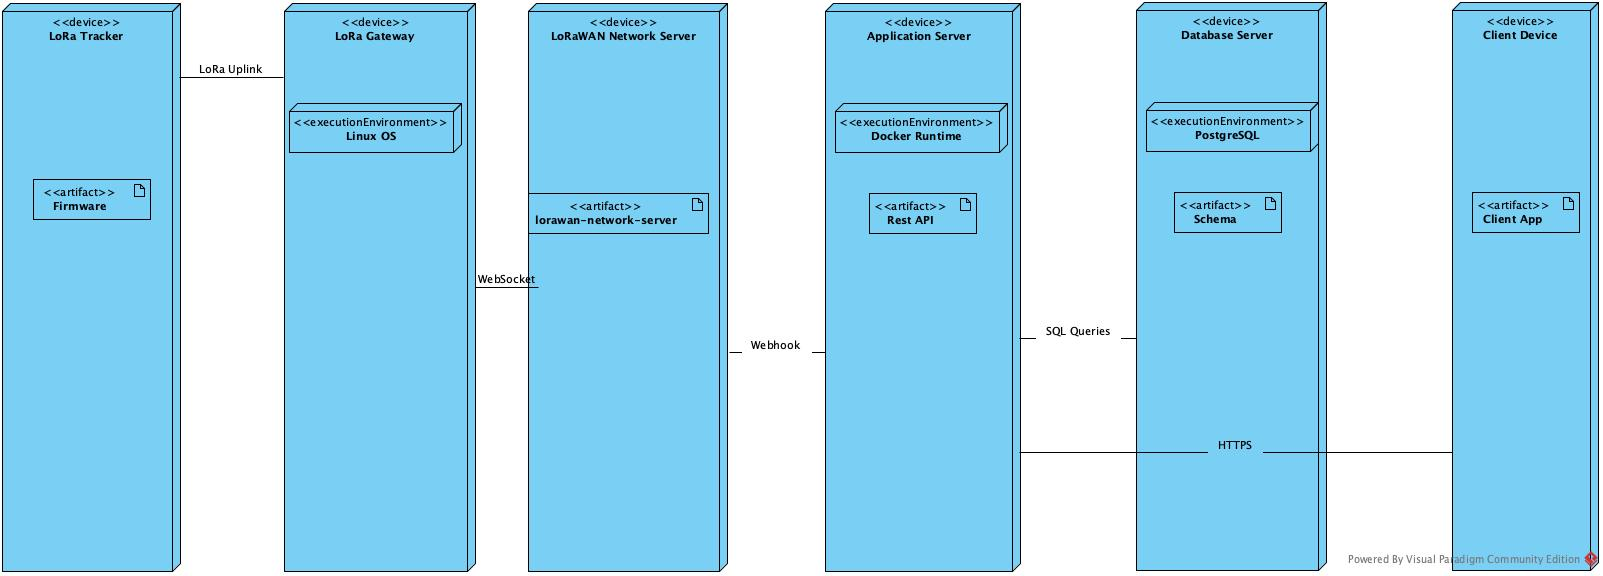
\includegraphics[width=0.7\textwidth]{png/systemOverview.jpg}
    \caption{System Diagram}
    \label{fig:SystemOverview}
\end{figure}

\subsection{Next Week's Plan}
Ryan will research open-source tracker designs; Roy will research scalability; Cory will research AWS-free workflows. We will continue debugging the LoRaWAN board.


%=======================================================
\section{Week Report 1 (09/05/2025)}
\label{sec:report1}

\subsection{Progress Made}
Ryan and Cory explored project ideas, consulted classmates and professors, and planned a decision timeline.

\subsection{Next Week's Plan}
Ryan will request continuation of his summer research project on LoRaWAN-based GPS tracking.

\subsection{Backup Plan}
If needed, the team may pivot to a “magic mirror” dashboard project driven by a Raspberry Pi.

